\documentclass[9pt,aspectratio=169,hyphens]{beamer}
\usepackage[append]{beamersubframe}
\usetheme{VK}
\setbeamertemplate{caption}[numbered]
% Mathematic Double-Stroke font
\usepackage{dsfont}
% Bold maths-mode
\usepackage{bm}
% Provides access to latin accents and many other characters in the Unicode lower plane.
% \usepackage{xunicode}
% extras?
\usepackage{xltxtra}
% Cyrillic language support
% \usepackage{xecyr}

% \usepackage{breakurl}
% \usepackage[hyphens]{url}
\usepackage{hyperref}  


\usepackage{tikz}
\usetikzlibrary{angles,quotes}
\usetikzlibrary{calc}
\usetikzlibrary{decorations.pathreplacing}
\usetikzlibrary{fadings}
\usetikzlibrary{arrows.meta}
\usetikzlibrary{shapes}
\usetikzlibrary{shapes.multipart}
\usetikzlibrary{patterns}
\pgfdeclarepatternformonly{south west lines}{\pgfqpoint{-0pt}{-0pt}}{\pgfqpoint{3pt}{3pt}}{\pgfqpoint{3pt}{3pt}}{
    \pgfsetlinewidth{0.4pt}
    \pgfpathmoveto{\pgfqpoint{0pt}{0pt}}
    \pgfpathlineto{\pgfqpoint{3pt}{3pt}}
    \pgfpathmoveto{\pgfqpoint{2.8pt}{-.2pt}}
    \pgfpathlineto{\pgfqpoint{3.2pt}{.2pt}}
    \pgfpathmoveto{\pgfqpoint{-.2pt}{2.8pt}}
    \pgfpathlineto{\pgfqpoint{.2pt}{3.2pt}}
    \pgfusepath{stroke}}


% default and example images
\usepackage{mwe}
%  Create tabular cells spanning multiple rows
\usepackage{multirow}

% turnipcite not suitable here, expects ToC to exist
% \usepackage{turnipcite}
\usepackage{csquotes}
\usepackage[british]{babel}
\usepackage[backend=biber,dateabbrev=false,style=alphabetic,
citestyle=authoryear,maxcitenames=1]{biblatex}
\addbibresource{mendeley_references.bib}
% \addbibresource{FinalReport/mendeley_export.bib}
\addbibresource{FinalReport/typ_FinalReport.bib}
\addbibresource{Presentation/references.bib}

\usepackage[font=normalsize,justification=centering]{caption}
\usepackage{tabularx}
\usepackage{siunitx}

\usepackage{environ}
% How to scale a tikzpicture to \textwidth
% https://tex.stackexchange.com/a/6391
% \makeatletter
% \newsavebox{\measure@tikzpicture}
% \NewEnviron{scaletikzpicturetowidth}[1]{%
%   \def\tikz@width{#1}%
%   \def\tikzscale{1}\begin{lrbox}{\measure@tikzpicture}%
%   \BODY
%   \end{lrbox}%
%   \pgfmathparse{#1/\wd\measure@tikzpicture}%
%   \edef\tikzscale{\pgfmathresult}%
%   \BODY
% }
% \makeatother

% biblatex authoryear brackets
% https://tex.stackexchange.com/a/16792
\makeatletter

\newrobustcmd*{\parentexttrack}[1]{%
  \begingroup
  \blx@blxinit
  \blx@setsfcodes
  \blx@bibopenparen#1\blx@bibcloseparen
  \endgroup}

\AtEveryCite{%
  \let\parentext=\parentexttrack%
  \let\bibopenparen=\bibopenbracket%
  \let\bibcloseparen=\bibclosebracket}

\makeatother

\usepackage[nofootnotes,release]{turniptodo}

\date[]{10th March 2020}
\title[]{Optimized Visualization of Fluid Simulations}
\author[]{Samuel Stark - u1800081 - 10th March 2020}

% \AtEndDocument{\usebeamertemplate{endpage}}

\usepackage{etoolbox}
\usepackage{listings}
% \usepackage{glslListings}

\definecolor{codegreen}{rgb}{0,0.6,0}
\definecolor{codegray}{rgb}{0.5,0.5,0.5}
\definecolor{codepurple}{rgb}{0.58,0,0.82}
\definecolor{backcolour}{rgb}{0.95,0.95,0.92}
\colorlet{numb}{magenta!60!black}
% \usepackage{courier}
\lstdefinestyle{mystyle}{
    basicstyle=\normalfont\ttfamily,
    backgroundcolor=\color{backcolour},   
    commentstyle=\color{codegreen},
    keywordstyle=\color{magenta},
    numberstyle=\tiny\color{codegray},
    stringstyle=\color{codepurple},
    basicstyle=\ttfamily\footnotesize,
    breakatwhitespace=false,         
    breaklines=true,                 
    captionpos=b,                    
    keepspaces=true,                 
    % numbers=left,
    % numberstyle=\scriptsize,
    % stepnumber=1,
    % numbersep=8pt,
    showstringspaces=false,
    breaklines=true,
    frame=lines,                  
    showspaces=false,                
    showtabs=false,                  
    tabsize=4
}
\lstset{style=mystyle}

% GLSL LISTINGS
%%
%% GLSL definition (c) 2020 Benno Bielmeier modified by Samuel Stark
%%
\lstdefinelanguage{GLSL}%
{%
    morekeywords={%
	% HLSL constants
		false,FALSE,NULL,true,TRUE,%
	% GLSL predefinde macro constant
		__LINE__,__FILE__,__VERSION__,GL_core_profile,GL_es_profile,GL_compatibility_profile,%
	% GLSL precision modifier
		precision,highp,mediump,lowp,%
	% GLSL control keywords
		break,case,continue,default,discard,do,else,for,if,return,switch,while,%
	% GLSL types
		void,bool,int,uint,float,double,vec2,vec3,vec4,dvec2,dvec3,dvec4,bvec2,bvec3,bvec4,ivec2,ivec3,ivec4,uvec2,uvec3,uvec4,mat2,mat3,mat4,mat2x2,mat2x3,mat2x4,mat3x2,mat3x3,mat3x4,mat4x2,mat4x3,mat4x4,dmat2,dmat3,dmat4,dmat2x2,dmat2x3,dmat2x4,dmat3x2,dmat3x3,dmat3x4,dmat4x2,dmat4x3,dmat4x4,sampler1D,sampler2D,sampler3D,image1D,image2D,image3D,samplerCube,imageCube,sampler2DRect,image2DRect,sampler1DArray,sampler2DArray,image1DArray,image2DArray,samplerBuffer,imageBuffer,sampler2DMS,image2DMS,sampler2DMSArray,image2DMSArray,samplerCubeArray,imageCubeArray,sampler1DShadow,sampler2DShadow,sampler2DRectShadow,sampler1DArrayShadow,sampler2DArrayShadow,samplerCubeShadow,samplerCubeArrayShadow,isampler1D,isampler2D,isampler3D,iimage1D,iimage2D,iimage3D,isamplerCube,iimageCube,isampler2DRect,iimage2DRect,isampler1DArray,isampler2DArray,iimage1DArray,iimage2DArray,isamplerBuffer,iimageBuffer,isampler2DMS,iimage2DMS,isampler2DMSArray,iimage2DMSArray,isamplerCubeArray,iimageCubeArray,atomic_uint,usampler1D,usampler2D,usampler3D,uimage1D,uimage2D,uimage3D,usamplerCube,uimageCube,usampler2DRect,uimage2DRect,usampler1DArray,usampler2DArray,uimage1DArray,uimage2DArray,usamplerBuffer,uimageBuffer,usampler2DMS,uimage2DMS,usampler2DMSArray,uimage2DMSArray,usamplerCubeArray,uimageCubeArray,struct,%
	% GLSL support variables
		gl_BackColor,gl_BackLightModelProduct,gl_BackLightProduct,gl_BackMaterial,gl_BackSecondaryColor,gl_ClipDistance,gl_ClipPlane,gl_ClipVertex,gl_Color,gl_DepthRange,gl_DepthRangeParameters,gl_EyePlaneQ,gl_EyePlaneR,gl_EyePlaneS,gl_EyePlaneT,gl_Fog,gl_FogCoord,gl_FogFragCoord,gl_FogParameters,gl_FragColor,gl_FragCoord,gl_FragData,gl_FragDepth,gl_FrontColor,gl_FrontFacing,gl_FrontLightModelProduct,gl_FrontLightProduct,gl_FrontMaterial,gl_FrontSecondaryColor,gl_InstanceID,gl_Layer,gl_LightModel,gl_LightModelParameters,gl_LightModelProducts,gl_LightProducts,gl_LightSource,gl_LightSourceParameters,gl_MaterialParameters,gl_ModelViewMatrix,gl_ModelViewMatrixInverse,gl_ModelViewMatrixInverseTranspose,gl_ModelViewMatrixTranspose,gl_ModelViewProjectionMatrix,gl_ModelViewProjectionMatrixInverse,gl_ModelViewProjectionMatrixInverseTranspose,gl_ModelViewProjectionMatrixTranspose,gl_MultiTexCoord0,gl_MultiTexCoord1,gl_MultiTexCoord2,gl_MultiTexCoord3,gl_MultiTexCoord4,gl_MultiTexCoord5,gl_MultiTexCoord6,gl_MultiTexCoord7,gl_Normal,gl_NormalMatrix,gl_NormalScale,gl_ObjectPlaneQ,gl_ObjectPlaneR,gl_ObjectPlaneS,gl_ObjectPlaneT,gl_Point,gl_PointCoord,gl_PointParameters,gl_PointSize,gl_Position,gl_PrimitiveIDIn,gl_ProjectionMatrix,gl_ProjectionMatrixInverse,gl_ProjectionMatrixInverseTranspose,gl_ProjectionMatrixTranspose,gl_SecondaryColor,gl_TexCoord,gl_TextureEnvColor,gl_TextureMatrix,gl_TextureMatrixInverse,gl_TextureMatrixInverseTranspose,gl_TextureMatrixTranspose,gl_Vertex,gl_VertexID,%
	% GLSL support constants
		gl_MaxClipPlanes,gl_MaxCombinedTextureImageUnits,gl_MaxDrawBuffers,gl_MaxFragmentUniformComponents,gl_MaxLights,gl_MaxTextureCoords,gl_MaxTextureImageUnits,gl_MaxTextureUnits,gl_MaxVaryingFloats,gl_MaxVertexAttribs,gl_MaxVertexTextureImageUnits,gl_MaxVertexUniformComponents,%
	% GLSL support functions
		abs,acos,all,any,asin,atan,ceil,clamp,cos,cross,degrees,dFdx,dFdy,distance,dot,equal,exp,exp2,faceforward,floor,fract,ftransform,fwidth,greaterThan,greaterThanEqual,inversesqrt,length,lessThan,lessThanEqual,log,log2,matrixCompMult,max,min,mix,mod,noise1,noise2,noise3,noise4,normalize,not,notEqual,outerProduct,pow,radians,reflect,refract,shadow1D,shadow1DLod,shadow1DProj,shadow1DProjLod,shadow2D,shadow2DLod,shadow2DProj,shadow2DProjLod,sign,sin,smoothstep,sqrt,step,tan,texture1D,texture1DLod,texture1DProj,texture1DProjLod,texture2D,texture2DLod,texture2DProj,texture2DProjLod,texture3D,texture3DLod,texture3DProj,texture3DProjLod,textureCube,textureCubeLod,transpose,%
	% GLSL struct member -> FixMe: Should have dot(.) as delimiter
		rgb
	},
	sensitive=true,%
	morecomment=[s]{/*}{*/},%
	morecomment=[l]//,%
	morestring=[b]",%
	morestring=[b]',%
	moredelim=*[directive]\#,%
	% keyword.control.hlsl
	moredirectives={define,defined,elif,else,if,ifdef,endif,line,error,ifndef,include,pragma,undef,warning,extension,version}%
}[keywords,comments,strings,directives]%

\lstset{basicstyle=\footnotesize\ttfamily,breaklines=true}
\lstset{framextopmargin=50pt,frame=bottomline}

\begin{document}
\maketitle

% \newenvironment{wideitemize}{\itemize\addtolength{\itemsep}{10pt}}{\enditemize}
            
\newenvironment{wideitemize}{\itemize\itemsep1.3em}{\enditemize}

\newcommand{\mytwocolumn}[3]{
    \begin{columns}[t,onlytextwidth]
        \begin{column}{#1\textwidth}
            #2
        \end{column}
        \begin{column}{\dimexpr\textwidth-(#1\textwidth)}
            #3
        \end{column}
    \end{columns}
}
\newcolumntype{C}{>{\centering\arraybackslash}X}

\section{Intro}

\begin{frame}{Disclaimer}
    \mytwocolumn{0.55}{
        \begin{wideitemize}
            \item The scope of this project is \emph{\Large huge!}
            \item 8,500 lines of code over 146 files (not including comments, blank space, libraries)
            \item I can't talk about everything interesting in 15 minutes.
            \item This is going to be a whistle-stop tour of the best bits.
            \item Ask me anything after the presentation and I can talk your ear off.
        \end{wideitemize}
    }{
    \vspace{-1.3em}
    \bgroup\begin{table}[t]
        \centering
        {\scriptsize
        \def\arraystretch{2}%  1 is the default, change whatever you need
        \begin{tabularx}{\textwidth}{|CC|}
            \hline
            Timestep calculations & Agnostic sim runners\\
            CUDA Unified Memory & Origin-aware pointers \\
            Parallel Reductions & CUDA Graphs \\
            \texttt{const \_\_restrict\_\_} & Frame allocation \\
            Image Layout Transfers & Vulkan Memory Model \\
            CUDA Warps & Push Constants \\
            Specialization Constants & Indirect Dispatch/Draw \\
            Indexed Rendering & Semaphores \\
            Fences & Vulkan Memory Allocation \\
            Memory Alignment & Atomic Variables \\
            \multicolumn{2}{|c|}{and more!} \\
            \hline
        \end{tabularx}
        }
        \caption{Interesting things I could talk about}
    \end{table}\egroup
    }
\end{frame}

\begin{frame}{CFD, Simulations, and High-Speeds}
    \begin{wideitemize}
        \item Equations modelling real-world phenomena have been around for centuries.
        \item Computational Fluid Dynamics programs (CFD) solve the Navier-Stokes equations to simulate fluid flow.
        \item Used in many fields:
        \begin{wideitemize}
            % \item Weather Simulation\todocite{https://www.futurelearn.com/info/courses/supercomputing/0/steps/24057}
            \item Aerodynamics \parencite{jameson2002}
            \item Fire Spread Modelling \parencite{Sullivan_2009}
            \item Entertainment Industry \parencite{article:FluidDynamicsOnBigScreen,paper:GameFluidSummary:medveckyreal}
        \end{wideitemize}
        \item Generally \textbf{interactive speeds} and \textbf{precise simulation} not pursued together.
    \end{wideitemize}
\end{frame}

\begin{frame}{Project Motivation}
    \begin{wideitemize}
        \item CS257 coursework presented a fluid simulation from \parencite{book:griebel1998numerical}, tasked students with optimizing it for a 6-core CPU.
        \item My solution \parencite{modules:aca257submission} ran 64x faster than the original, and 7.9x faster than real-time, on the given input data.
        \item But the simulation was still limited:
        \begin{wideitemize}
            \normalsize
            \item We were prevented from running it on a GPU for greater speedups.
            \item Results could only be visualized after the fact, even though it was fast enough to render in real time.
        \end{wideitemize}
    \end{wideitemize}
\end{frame}

\begin{frame}{Project Goals/Achievements}
    \begin{center}
        {
        \LARGE
        \textbf{Port the simulation to the GPU.}\\
        \vspace{1em}
        \textbf{Exploit the speedup to improve accuracy and increase sim resolution.}\\
        \vspace{1em}
        \textbf{Intuitively visualize the simulation in real time.\footnote{Use games industry techniques for efficient rendering.}}
        }
        
        %\footnote{Specifically a `tightly-coupled in-situ visualization'\todocite{tightly-coupled in-situ}} in Vulkan
        
        \vfill\null
        {\Large All goals were achieved!}
        
        \vfill\null
        
        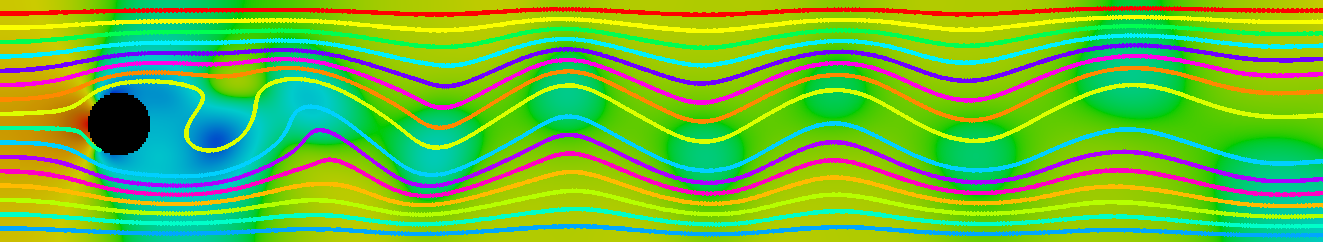
\includegraphics[width=0.7\textwidth]{Presentation/images/viz_particles.png}
        % \begin{tabularx}{\textwidth}{CCC}
        %     \todomark{Figures for speedup} & \todomark{example accuracy} & \todomark{Visualization example} \\
        % \end{tabularx}
    \end{center}
    % \begin{enumerate}
    %     \item Port the simulation to the GPU without significant loss of accuracy.
    %     \item Increase the simulation accuracy.
    %     \item 
    % \end{enumerate}
\end{frame}

% CFDs & Simulation
% - Modelling natural phenomena has been around for ages (Navier-Stokes equations from XX years ago).
% - CFDs are programs that compute results for Navier-Stokes to simulate how fluid moves.
% - Variety of uses
% - generally not required to be at interacive speeds.
%   - when you do, you don't integrate precisely "The model  would  not  be  accurate  enoughfor most engineering applications" [Stam99]

% Vizualization
% Another important property is visualizing the outputs of a simulation.
% Fluid visualization has stagnated - noticed in 2004, still the case today.
% current methods used in Autodesk CFD date back to XX years ago.
% even methods used for viz are getting old
% VTK still uses OpenGL 2 from 2004.

% \begin{frame}{Visualization}
    
% \end{frame}

% Motivation
% ACA coursework last year was to optimize a fluid simulation.
% I optimized it from X to Y, top in class
% But we can go faster
%    - GPU
% and we can visualize it better
%    - in-situ
%    - viz will need to be fast if we're keeping the simulation fast.
%    - use games background, real-time-rendering techniques.
%    - focus on intuive viz
% \input{Presentation/sections/10_background}
% \input{Presentation/sections/20_key_idea}
\section{Simulation}
\subsection{Overview}

\begin{frame}{Simulation Overview}
    \mytwocolumn{0.6}{
        \begin{wideitemize}
            \item Simulation code preserved from CS257 submission.
            \item Simulates ``laminar flows of viscous, incompressible fluids''.
            \item Fluid is represented by a 2D array of cells.
            \item Fluid flows around static `obstacle' cells.
            \item Generates values for velocity $(u, v)$ and relative pressure $p$.
        \end{wideitemize}
    }{
        \begin{figure}
            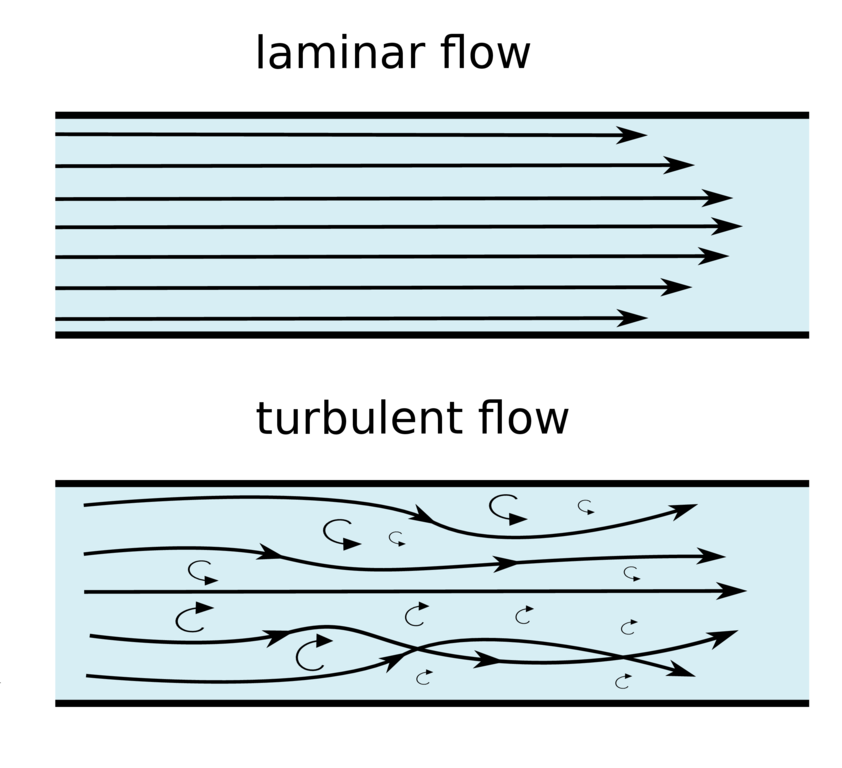
\includegraphics[width=\textwidth]{Presentation/images/sketch-laminar-flow-turbulent-flow.png}
            \caption{Laminar vs. turbulent fluid flow. Reproduced from cfdsupport.com}
            \label{fig:laminar_flow}
        \end{figure}
    }
\end{frame}

% \begin{frame}{Simulation Overview}
%     \mytwocolumn{0.6}{
%         \begin{wideitemize}
%             \item Simulation code preserved from CS257 submission.
%             \item 2D simulation of ``laminar flows of viscous, incompressible fluids''.
%             \item Generates values for velocity $(u, v)$ and relative pressure $p$.
%         \end{wideitemize}
%     }{
%         \input{FinalReport/Ch20Research/figures/staggered_grid}
%     }
% \end{frame}

\begin{frame}{Simulation Structure}
    \mytwocolumn{0.6}{
        \begin{wideitemize}
            \item Simulation runs in `ticks', each representing a discrete timestep $\delta{t}$.
            \item Each `tick' has multiple sequential execution stages.
            \item Each stage has been optimized to be embarassingly parallel.
            \item Poisson Solver runs for a constant amount of iterations each tick.
        \end{wideitemize}
    }{
        \begin{figure}
            \centering

        \begin{tikzpicture}[
        scale=0.8, every node/.style={scale=0.8},
        stage/.style={minimum height = 2.5em, draw, anchor=north}
        ]
            \newcommand{\stagesep}{-0.4};
            \node[stage](s1) at (0,0) {Compute $\delta{t}$};
            \node[stage](s2) at ($(s1.south) + (0,\stagesep)$) {Compute Tentative Velocity};
            \node[stage](s3) at ($(s2.south) + (0,\stagesep)$) {Compute Poisson RHS};
            \node[stage](s4) at ($(s3.south) + (0,\stagesep)$) {Poisson Solver};
            % \node[stage](s5) at ($(s4.south) + (0,-0.6)$) {Poisson Iteration \#2};
            % \node[stage](s6) at ($(s5.south) + (0,-0.6)$) {...};
            % \node[stage](s7) at ($(s6.south) + (0,-0.6)$) {Poisson Iteration \#N};
            \node[stage](s8) at ($(s4.south) + (0,\stagesep)$) {Update Velocity};
            \node[stage](s9) at ($(s8.south) + (0,\stagesep)$) {Boundary Conditions};

            \draw[thick, ->] (s4.east) arc (0:-330:-0.4cm);% syntax (starting point coordinates) arc (starting angle:ending angle:radius)
            \node at ($(s4.east) + (2cm, 0)$){$N$ {}iterations}; 

            \draw[-latex] (s1.south) -- (s2.north);
            \draw[-latex] (s2.south) -- (s3.north);
            \draw[-latex] (s3.south) -- (s4.north);
            \draw[-latex] (s4.south) -- (s8.north);
            % \draw[-latex] (s5.south) -- (s6.north);
            % \draw[-latex] (s6.south) -- (s7.north);
            % \draw[-latex] (s7.south) -- (s8.north);
            \draw[-latex] (s8.south) -- (s9.north);
        \end{tikzpicture}
        \caption{An example simulation tick}
        \label{fig:my_label}
    \end{figure}
    }
\end{frame}

\begin{frame}[fragile]{Simulation Kernels}
    % \begin{columns}\begin{column}{0.4\textwidth}
        \begin{wideitemize}
            \item This maps incredibly well to CUDA `kernels'\footnote{\url{https://docs.nvidia.com/cuda/cuda-c-programming-guide/index.html\#kernels}}.
            \item Each stage is implemented as one or more kernels, run over every element in parallel.
        \end{wideitemize}
    % \end{column}
    % \begin{column}{0.7\textwidth}
    \begin{figure}[b]
        \centering

        \lstset{language=c,keywords={__global__},
    keywordstyle=[1]\color{blue}}
        \begin{lstlisting}
// Computing delta-t is done slightly differently (ask me about it at the end!)
        
__global__ void computeTentativeVelocity_apply(...);
__global__ void computeTentativeVelocity_postproc_vertical(...);
__global__ void computeTentativeVelocity_postproc_horizontal(...);

__global__ void computeRHS_1per(...);

__global__ void poisson_single_tick(...);

__global__ void updateVelocity_1per(...);

__global__ void boundaryConditions_preproc_vertical(...);
__global__ void boundaryConditions_preproc_horizontal(...);
__global__ void boundaryConditions_apply(...);
__global__ void boundaryConditions_inputflow_west_vertical(...);\end{lstlisting}

        % \caption{CUDA Kernel Definitions}
    \end{figure}
    % \end{column}\end{columns}
\end{frame}

\begin{frame}{CUDA Unified Memory}
    % \todomark{Ask me about unified memory afterwards}
    
    \mytwocolumn{0.5}{
        \begin{wideitemize}
            \item CUDA provides Unified Memory allocations\footnotemark
            \item Paged between the Host and Device on-demand.
            \item Same performance as normal GPU memory when present on the device.
            \item Used to mix CPU and GPU implementations while testing and debugging.
        \end{wideitemize}
    }{
        \begin{figure}
            \centering
            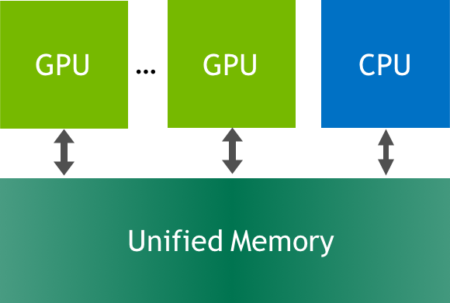
\includegraphics[width=0.7\textwidth]{Presentation/images/unified_memory_smol.png}
            % \caption{Caption}
            % \label{fig:my_label}
        \end{figure}
    }
    
    \footnotetext{\url{https://developer.nvidia.com/blog/unified-memory-cuda-beginners/}}
    
    % \vfill\null
    % \begin{center}
    %     Ask me about Simulation Memory Allocation at the end!
    % \end{center}
    % CUDA allows Unified Memory\parencite{https://developer.nvidia.com/blog/unified-memory-cuda-beginners/} to be allocated
    % Paged between Host and Device on-demand 
    % Allows incremental development of GPU kernels by using CPU code for kernels which haven't been ported yet.
    
    % image from {https://developer.nvidia.com/maximizing-unified-memory-performance-cuda-0}
\end{frame}

\subsection{Optimizations}

\begin{frame}[fragile]{\texttt{const \_\_restrict\_\_} pointers}
    % CUDA has a ``read-only data cache'' {https://docs.nvidia.com/cuda/cuda-c-programming-guide/index.html#global-memory-3-0}
    % Use `const __restrict__ T*` pointers to show the compiler which data is read-only
    % Developed a standardized kernel setup to ensure pointers are all __restrict__ed
    % Speeds up execution time\parencite{const restrict thingy}
    
    \begin{minipage}{0.5\textwidth}
        \begin{wideitemize}
        \item CUDA exposes a fast ``read-only data cache''\footnotemark{}.
        \item To ensure the compiler knows memory is read only, use the \texttt{const} and \texttt{\_\_restrict\_\_} qualifiers on all pointers.
        \item Shown to speed up execution times in \parencite{10.1145/3238147.3241533}.
        \end{wideitemize}
    \end{minipage}\hfill%
    \begin{minipage}{0.4\textwidth}
    \begin{figure}[b]
        \centering

        \lstset{language=c,keywords={template,typename,using},keywordstyle=[1]\color{blue}}
        \begin{lstlisting}
template<typename T>
using in_matrix = 
    const T* const __restrict__;

template<typename T>
using out_matrix = 
    T* const __restrict__;\end{lstlisting}
        \caption{Helper templates used in kernel definitions}
    \end{figure}
    \end{minipage}
    % }
    \footnotetext{\url{https://docs.nvidia.com/cuda/cuda-c-programming-guide/index.html\#global-memory-3-0}}
    
    \vfill\null
    \begin{center}
        Ask me about \texttt{const \_\_restrict\_\_} pointers at the end!
    \end{center}
    
    % Detail slide:
    % in_matrix<T> out_matrix<T>
    % Why out_matrix<T> needs to be __restrict__ too
\end{frame}

\begin{frame}{Parallel Reductions}
    % \todomark{Ask me about unified memory afterwards}
    
    \mytwocolumn{0.6}{
        \begin{wideitemize}
            \item Computing $\delta{t}$ requires the maximum values of $u, v$.
            \item We can do this in parallel on the GPU!
            \item Find the values on the GPU, then copy them to the CPU to calculate $\delta{t}$.
            \item Implementation taken from \parencite{CUDAParallelReduction}.
        \end{wideitemize}
    }{
        \begin{figure}
            \centering
            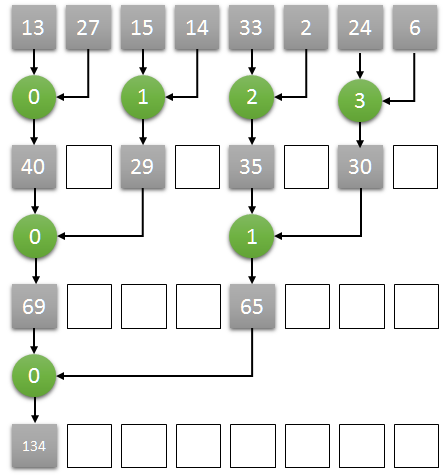
\includegraphics[width=0.7\textwidth]{Presentation/images/parallel_reduce.png}
            \caption{Example of parallel reduction for sum.\\Reproduced from \href{https://www.eximiaco.tech/en/2019/06/10/implementing-parallel-reduction-in-cuda/}{eximiaco.tech}}
            % \label{fig:my_label}
        \end{figure}
    }
    
    % \vfill\null
    % \begin{center}
    %     Ask me about Simulation Memory Allocation at the end!
    % \end{center}
    % CUDA allows Unified Memory\parencite{https://developer.nvidia.com/blog/unified-memory-cuda-beginners/} to be allocated
    % Paged between Host and Device on-demand 
    % Allows incremental development of GPU kernels by using CPU code for kernels which haven't been ported yet.
    
    % image from {https://developer.nvidia.com/maximizing-unified-memory-performance-cuda-0}
\end{frame}

\begin{frame}[fragile]{CUDA Graphs}
    % \todomark{Go in depth}
    % Profiling showed GPU bubbles between poisson iterations
    % cuda launches supposed to be asynchronous, but behaviour looks closer to synchronous
    % Instead of launching N times, record a CUDA graph containing N iterations, invoke that once.
    % Avoids CPU overhead, shows 2x speedup in profiler
    
    \begin{wideitemize}
        \item CPU overhead when launching Poisson kernels caused large GPU bubbles.
        \item Instead of launching N times, record a CUDA Graph\footnote{\url{https://developer.nvidia.com/blog/cuda-graphs/}} that runs N iterations, and launch it once.
        \item Theoretical 2x speedup.
    \end{wideitemize}
    
    \vfill\null
    \begin{minipage}{0.48\textwidth}
        \begin{lstlisting}
for (int i = 0; i < 100; i++) {
    launch poisson on stream;
}\end{lstlisting}
    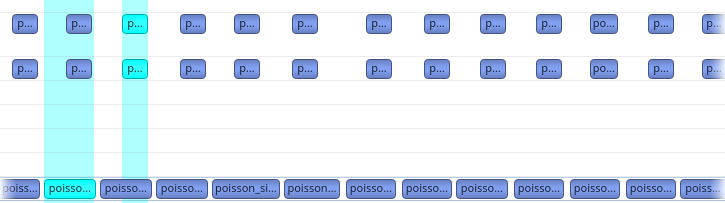
\includegraphics[width=\textwidth]{Presentation/images/cudagraphs_before.png}
    \begin{center}
        Individual Launches
    \end{center}
    \end{minipage}\hfill%
    \begin{minipage}{0.48\textwidth}
    \begin{lstlisting}
(record poisson100Iters if not present)

cudaGraphLaunch(poisson100Iters, stream);
\end{lstlisting}
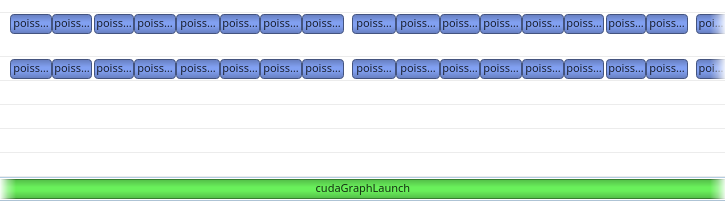
\includegraphics[width=\textwidth]{Presentation/images/cudagraphs_after.png}
        \begin{center}
        With CUDA Graphs
        \end{center}
    \end{minipage}
    % Potential cause
    % launches took more time than the actual execution
    % diminishing returns when kernels take longer

\end{frame}
% Porting multithreaded C to CUDA
% problems are all embarassingly parallel
% Red-black used (don't need to explain thoroughly
% Already optimized for parallelism, move to CUDA was easy.
% had to un-vectorize, as GPUs don't have vector registers

% Unified memory?
% CUDA can allocate "unified memory" 
% Usable from CPU and GPU without having to manually transfer
% Automatically pages from one side to the other
% Great for initially creating the algorithm

% CUDA-specific optimizations
% const __restrict__ pointers
% CUDA has special, fast memory for data that is guaranteed not to change.
% All functions have separate inputs and outputs, so this memory would be very helpful
% Use const to ensure the compiler knows it can't be written to, __restrict__ to tell the compiler that no other pointers point to the same data.
% These guarantees allow the compiler to use the special memory TODO find the name
% Shown in [] to have distinct benefits.

% Implemented by using in_matrix<T>, out_matrix<T> for all arguments to kernels
% C++ support in CUDA converts these to const __restrict__ pointers

% Cuda Graphs
% Profiling showed many pipeline bubbles between Poisson iterations
% Issue is with dispatching kernels:
%  dispatching is asynchrnous, but you can only dispatch so many things before you have to wait?
%  or was the kernel executing faster than the CPU managed to dispatch them?
% either way - had to wait for the CPU to dispatch the next kernel.
% CUDA graphs[] allow you to record a set of actions, then enqueue them all at once.
% This reduces CPU overhead of poisson to 0, removing utilization bubbles and halving the time taken. (other kernels were not added to the graph as future extensions were planned)

% CUDA reductions
% the simulation requires finding the maximum value in arrays
% use a parallel reduction to do this on the GPU, and avoid transferring data to the CPU and back.

\section{Visualization}
\subsection{Research}

\begin{frame}{Visualization Research I}
% Academia hasn't innovated new methods in ages. Does try to speed things up.
% Noted in 2004, seems to still be true now.
% MET Office does 
% Our specific kind of visualization (in-situ visualization) emerged in the 2010s, but again this only focuses on speedup methods, hooking things together.
\begin{wideitemize}
    \item This program is an example of `tightly-coupled in-situ visualization' \parencite{kress2017situ}.
    \item Academia hasn't recently innovated in fluid visualization, only in methods for running faster such as \parencite{efficientStreamConstruction}.
    \item This was noted in \parencite{vizRole2004}, which states `feature detection' would be a key element going forward rather than new visualization methods.
\end{wideitemize}
\end{frame}

\begin{frame}{Visualization Research II}
\mytwocolumn{0.5}{
\begin{wideitemize}
    \item Industry seems to match this assessment.
    \item Tools such as Autodesk CFD, Tecplot, ParaView all visualize data with the same general methods...
    \item but they allow the data to be \emph{filtered} to extract relevant values.
    \item Methods can be combined to show a range of information.
\end{wideitemize}
}{
    \begin{figure}
        \centering
        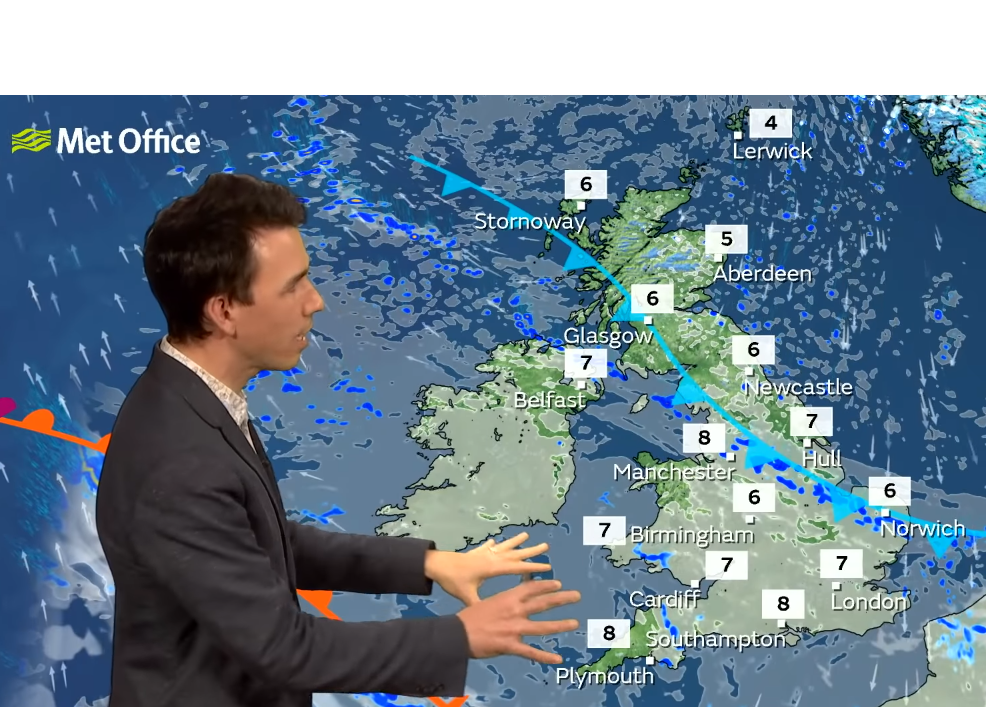
\includegraphics[width=0.7\textwidth]{Presentation/images/weather.PNG}
        \caption{Weather Forecast showing wind speed, weather fronts, and cloud cover.\footnotemark{}}
    \end{figure}
}
\footnotetext{\url{https://youtu.be/y_1--MkiNjQ}, Met Office 10 Day Trend for March 3rd.}
% Look to industry for potential innovation.
% Selected Autodesk CFD for a fluid-focused visualization.
% Found X methods of interest
% list them
% All have been present from 195X, confirming belief.
\end{frame}

\newcommand{\vizresearch}[3]{
\begin{frame}{Visualization Research}
    % \framesubtitle{What can Autodesk CFD do?}
    % \begin{columns}[t,onlytextwidth]
    %     \begin{column}{0.5\textwidth}
    %         {\Large #1}
    %         \vspace{2em}
    %         #2
    %     \end{column}
    %     \begin{column}{0.3\textwidth}
    %         #3
    %     \end{column}
    % \end{columns}
    
    \framesubtitle{What can Autodesk CFD do?}
    \begin{minipage}{0.5\textwidth}
        {\Large #1}
        \vspace{2em}
        #2
    \end{minipage}\hfill%
    \begin{minipage}{0.48\textwidth}
        #3
    \end{minipage}
\end{frame}
}

\vizresearch{Result Planes - Scalar}{
    % \todocite{http://help.autodesk.com/view/SCDSE/2019/ENU/?guid=GUID-AA40D02F-8CBC-4F78-A3C8-CEF30E05522B}
    \begin{wideitemize}
        \item Place a plane in 3D space
        \item Select a scalar quantity (pressure, temperature etc.)
        \item The cross-section of the model shows the selected quantity, with a color scale
        % \todomark{matplotlib jet colormap}
    \end{wideitemize}
}{
\begin{figure}
    \centering
    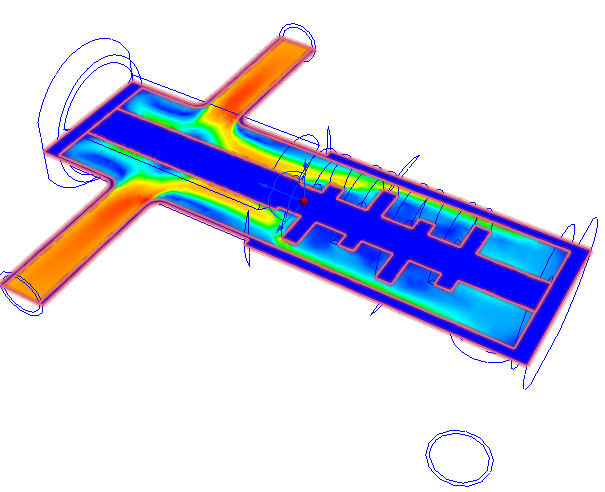
\includegraphics[width=0.9\textwidth]{Presentation/images/autodesk_cfd_results_planes_scalar.png}
\end{figure}
}

\vizresearch{Result Planes - Vector}{
    % \todocite{http://help.autodesk.com/view/SCDSE/2019/ENU/?guid=GUID-AA40D02F-8CBC-4F78-A3C8-CEF30E05522B}
    \begin{wideitemize}
        \item Place a plane in 3D space
        \item Select a \emph{vector} quantity (velocity etc.)
        \item The cross-section of the model shows a vector field of the selected velocity.
    \end{wideitemize}
}{
\begin{figure}
    \centering
    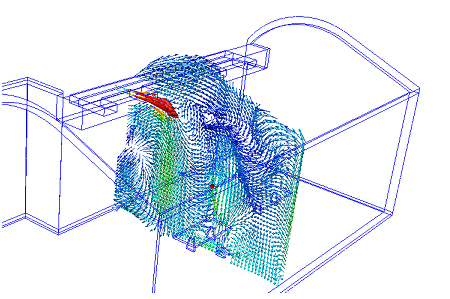
\includegraphics[width=0.9\textwidth]{Presentation/images/autodesk_cfd_results_planes_vector.png}
\end{figure}
}

\vizresearch{Isosurfaces}{
% \todocite{http://help.autodesk.com/view/SCDSE/2019/ENU/?guid=GUID-9D0D1D9C-C087-42A5-87F6-24F6A8530244}
    \begin{wideitemize}
        \item Select a scalar quantity $X$.
        \item Select a value $X = x$.
        \item This surface is displayed with a color based on another quantity $Y$.
        \item A vector quantity can also be added to the surface.
    \end{wideitemize}
}{
\begin{figure}
    \centering
    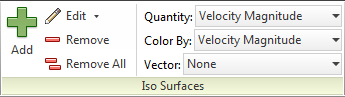
\includegraphics[width=0.6\textwidth]{Presentation/images/isosurface_control.png}
\end{figure}
\begin{figure}
    \centering
    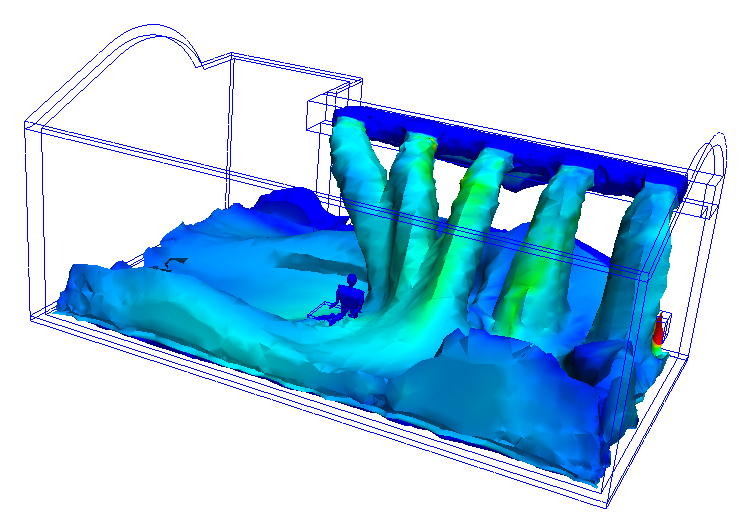
\includegraphics[width=0.9\textwidth]{Presentation/images/isosurface.png}
\end{figure}
}

\vizresearch{Isovolumes}{
% \todocite{http://help.autodesk.com/view/SCDSE/2019/ENU/?guid=GUID-9D0D1D9C-C087-42A5-87F6-24F6A8530244}
    \begin{wideitemize}
        \item Select a scalar quantity $X$.
        \item Select a \emph{range} $x_{min} \leq X \leq x_{max}$.
        \item This \emph{volume} is displayed with a color based on another quantity $Y$.
        \item A vector quantity can also be added to the \emph{volume}.
    \end{wideitemize}
}{
\begin{figure}
    \centering
    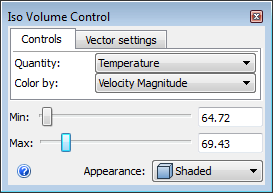
\includegraphics[width=0.5\textwidth]{Presentation/images/isovolume_ui.png}
\end{figure}
\begin{figure}
    \centering
    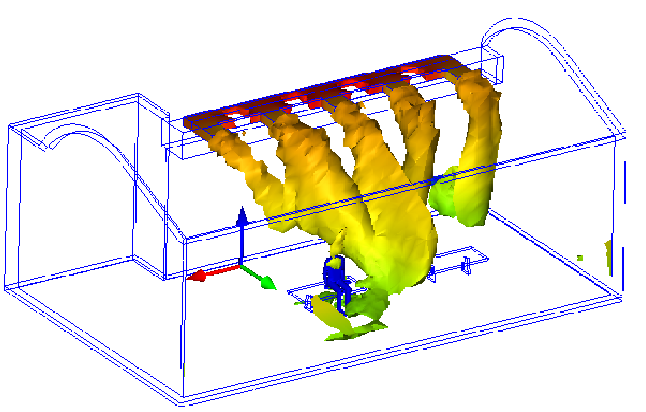
\includegraphics[width=0.9\textwidth]{Presentation/images/isovolume_noui.png}
\end{figure}
}

\vizresearch{Particles}{
% \todocite{http://help.autodesk.com/view/SCDSE/2019/ENU/?guid=GUID-9EBC3C73-AB3B-4341-BBDF-58601024BD7C}
    \begin{wideitemize}
        \item Place particle spawn points (`seeds').
        \item Select a scalar quantity to display, or a solid color.
        \item Points along the particle paths show the specified quantity.
        \item Can choose many kinds of path:
        \begin{itemize}
            \item Cylinders
            \item Ribbons
            \item Comets
            \item etc.
        \end{itemize}
    \end{wideitemize}
}{
\begin{figure}
    \centering
    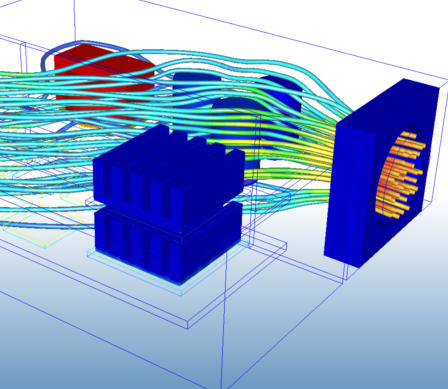
\includegraphics[width=0.9\textwidth]{Presentation/images/particle_traces.jpg}
\end{figure}
}

% \begin{frame}{Visualization Research II - Weather Reports}
% % Met office layers many effects on top of each other.
% \mytwocolumn{0.5}{
% \begin{wideitemize}
%     \item The MET office is an example of an intuitive fluid visualization.
%     \item 
% \end{wideitemize}
% }
% \end{frame}

\subsection{Design}

\begin{frame}{Selected Features}
% Select 3 layers, which can be overlayed on each other, like the weather report.

% Take iso-shapes as the 2D equivalent of isovolumes
% For both scalar and vector processing
% Add particles
%  failed to add particle trails
        Separate the visualization into layers:
        \vspace{1em}

        \begin{wideitemize}
            \item Background
            \item Scalar Quantity
            \begin{itemize}
                \item Display a quantity $X$ using a colormap when $x_{min} \leq X \leq x_{max}$
                \item Allow the user to select a range, or calculate a range containing all values
                \item Equivalent to Results Plane (Scalar) + 2D Isovolume
            \end{itemize}
            \item Vector Quantity 
            \begin{itemize}
                \item Display a vector field of $X$ when $x_{min} \leq X \leq x_{max}$
                \item Allow the user to select a range, or calculate a range containing all values
                \item Equivalent to Results Plane (Vector) + 2D Isovolume
            \end{itemize}
            \item Particles
                \begin{itemize}
                    \item Editable `seeds'
                    \item Planned for particle trace options, didn't have time.
                \end{itemize}
        \end{wideitemize}
    % }{
    % daui
    % }
\end{frame}

\begin{frame}{Anatomy of a Frame}
% "Mention zero copy"
% Need to mention "need compute + graphics"
% Include CPU recording

    \makebox[\textwidth][c]{
    \begin{tikzpicture}[
    scale=0.9, every node/.style={scale=0.9},
fixedrect/.style={rectangle,draw,minimum height=4em,anchor=west,text width=2cm,align=center},
]
        \node[label=west:{GPU},align=right](gpu) at (0,0){};
        \node[label=west:{CPU 0},align=right](c0) at (0,-4em){};
        \node[label=west:{CPU 1},align=right](c1) at (0,-8em){};

        \node[fixedrect, text width=1.5cm, path fading = west](gpu_viz_g_old) at (gpu){Viz \\N-1};%\\[Vulkan]};
        \node[fixedrect, text width=6cm](gpu_sim) at (gpu_viz_g_old.east){Simulation\\N};%\\[CUDA]};
        \node[fixedrect, text width=2cm](gpu_viz_c) at (gpu_sim.east){Viz Compute\\N};%\\[Vulkan]};
        \node[fixedrect, text width=2cm](gpu_viz_g) at (gpu_viz_c.east){Viz Graphics\\N};%\\[Vulkan]};
        \node[fixedrect, text width=2cm, path fading = east](gpu_sim_next) at (gpu_viz_g.east){Sim\\N+1};%\\[Vulkan]};

        \node[fixedrect, text width=4.5cm](c0_sim) at (c0 -| gpu_sim.west){Launch Sim Kernels};%\\[Vulkan]};
        \node[fixedrect, text width=3cm](c1_record) at (1,0 |- c1){Record Visualization};%\\[Vulkan]};

        % \draw[-latex] (c0_sim.north -| 1,0) -- (gpu_sim.west);
        \draw[-latex] (c1_record.east) -| (gpu_viz_c.south west);
        \draw[-latex] (c0) -- (c1_record.west);
        % \draw[-latex] (c1_record.east) -- (gpu_viz.south);
        % \draw[-latex] (c1_record.east) -| (gpu_viz.south);
        % \draw[-latex] (c1_record.east) -| (gpu_viz.south);
    \end{tikzpicture}
    }

    \vfill\null
    \begin{wideitemize}
        % \item CPU 0 (main thread) starts a worker thread to record what the GPU will do for the visualization.
        \item CPU 0 launches the simulation, which requires some CPU/GPU sync at the start.
        \item CPU 1 enqueues the visualization work to start right after the simulation.
        \item Sim and Visualization share memory, architecture is zero-copy.
        \item Maintains near-100\% GPU Utilization.
    \end{wideitemize}
    % Key point is that the "Record Visualization" may overlap with a previous viz frame, so it can't look at any GPU memory.
\end{frame}

\begin{frame}{GPU Synchronization}
% Semaphores
    \makebox[\textwidth][c]{
    \begin{tikzpicture}[
            scale=0.9, every node/.style={scale=0.9},
        fixedrect/.style={rectangle,draw,minimum height=4em,anchor=west,text width=2cm,align=center},
        ]
        \node[label=west:{GPU - CUDA},align=right](cuda) at (0,0){};
        \node[label=west:{GPU - Vulkan},align=right](vulkan) at (0,-4em){};

        \node[fixedrect, text width=1.5cm, path fading = west](vc_old) at (vulkan){Viz Comp\\N-1};
        \node[fixedrect, text width=2cm](vg_old) at (vc_old.east){Viz Graphics\\N-1};
        \node[fixedrect, text width=6cm](sim) at (vc_old.east |- cuda){Simulation\\N};%\\[CUDA]};
        \node[fixedrect, text width=2cm](vc) at (sim.east |- vulkan){Viz Compute\\N};%\\[Vulkan]};
        \node[fixedrect, text width=2cm](vg) at (vc.east){Viz Graphics\\N};
        \node[fixedrect, text width=4cm, anchor=west,path fading = east](sim_new) at (vg.west |- cuda){Sim\\N+1};
        
        \draw[ultra thick,black,-Triangle] (vc.south west) -- (sim.north east) |- ++(0.25,0.5) ;
            % node[east,text width=2cm,anchor=west]{Vulkan/CUDA Shared Semaphore};
        \draw[ultra thick,black,-Triangle] (vc_old.south east) -- (sim.north west) |- ++(0.25,0.5) ;
            % node[east,text width=2cm,anchor=west]{Vulkan/CUDA Shared Semaphore};
        \draw[ultra thick,black,-Triangle] (vg.south west) -- (sim_new.north west) |- ++(0.25,0.5) ;
            % node[east]{};
            
        % \draw[ultra thick,black,-Triangle] (vg.south west) -- (vg.north west) |- ++(0.25,0.5) ;
            % node[text width=2cm,anchor=north,below=5pt]{Vulkan-Only};

            
        % \node[text width = 3cm,align=center,anchor=north,below=10pt](sem_label) at (sim.south |- vc.south){Vulkan/CUDA Shared};
        % \draw[dashed](sem_label.north east) -- (vc.south west);
        % \draw[dashed](sem_label.north west) -- (vg_old.south east);
        
        % \node[text width = 3cm,align=center,anchor=north,below=10pt](vk_label) at (vg.south west){Vulkan-Only};
        % \draw[dashed](vk_label.north) -- (vc.south east);

        \end{tikzpicture}
    }

    \vfill\null
    
    \begin{wideitemize}
        \item Synchronization between overall workloads is performed via \emph{semaphores}\footnote{\url{https://www.khronos.org/registry/vulkan/specs/1.2-extensions/man/html/VkSemaphore.html}}.
        \item One workload waits on a semaphore until another workload signals it.
        \item Compute workloads cannot overlap on my graphics card\footnote{Running parallel compute workloads was introduced in \parencite{nvidiaAmpereWhitepaper}}
        \item Simulation and Viz Graphics \emph{could} overlap, but don't in practice.
        % \item More semaphores used in the program for `present' logic.
    \end{wideitemize}
\end{frame}

\begin{frame}{GPU Synchronization - Less Misleading}
% Semaphores
    \makebox[\textwidth][c]{
    \begin{tikzpicture}[
            scale=0.9, every node/.style={scale=0.9},
        fixedrect/.style={rectangle,draw,minimum height=4em,anchor=west,text width=2cm,align=center},
        ]
        \node[label=west:{GPU - CUDA},align=right](cuda) at (0,0){};
        \node[label=west:{GPU - Vulkan},align=right](vulkan) at (0,-4em){};

        \node[fixedrect, text width=1.5cm, path fading = west](vc_old) at (vulkan){Viz Comp\\N-1};
        \node[fixedrect, text width=2cm](vg_old) at (vc_old.east){Viz Graphics\\N-1};
        \node[fixedrect, text width=6cm](sim) at (vc_old.east |- cuda){Simulation\\N};%\\[CUDA]};
        \node[fixedrect, text width=2cm](vc) at (sim.east |- vulkan){Viz Compute\\N};%\\[Vulkan]};
        \node[fixedrect, text width=2cm](vg) at (vc.east){Viz Graphics\\N};
        \node[fixedrect, text width=4cm, anchor=west,path fading = east](sim_new) at (vg.west |- cuda){Sim\\N+1};
        
        \draw[ultra thick,black,-Triangle] (vc.south west) -- (sim.north east) |- ++(0.25,0.5) ;
            % node[east,text width=2cm,anchor=west]{Vulkan/CUDA Shared Semaphore};
        \draw[ultra thick,black,-Triangle] (vc_old.south east) -- (vc_old.east) -- (sim_new.west) -- (sim_new.north west) |- ++(0.25,0.5) ;
            % node[east,text width=2cm,anchor=west]{Vulkan/CUDA Shared Semaphore};
        \draw[ultra thick,black,-Triangle] (vg.south west) -- (vg.north west) |- ++(0.25,0.2) ;
            % node[east]{};
            
        % \draw[ultra thick,black,-Triangle] (vg.south west) -- (vg.north west) |- ++(0.25,0.5) ;
            % node[text width=2cm,anchor=north,below=5pt]{Vulkan-Only};

            
        % \node[text width = 3cm,align=center,anchor=north,below=10pt](sem_label) at (sim.south |- vc.south){Vulkan/CUDA Shared};
        % \draw[dashed](sem_label.north east) -- (vc.south west);
        % \draw[dashed](sem_label.north west) -- (vg_old.south east);
        
        % \node[text width = 3cm,align=center,anchor=north,below=10pt](vk_label) at (vg.south west){Vulkan-Only};
        % \draw[dashed](vk_label.north) -- (vc.south east);

        \end{tikzpicture}
    }

    \vfill\null
    
    \begin{wideitemize}
        \item Synchronization between overall workloads is performed via \emph{semaphores}\footnote{\url{https://www.khronos.org/registry/vulkan/specs/1.2-extensions/man/html/VkSemaphore.html}}.
        \item One workload waits on a semaphore until another workload signals it.
        \item Compute workloads cannot overlap on my graphics card\footnote{Running parallel compute workloads was introduced in \parencite{nvidiaAmpereWhitepaper}}
        \item Simulation and Viz Graphics \emph{could} overlap, but don't in practice.
        % \item More semaphores used in the program for `present' logic.
    \end{wideitemize}
\end{frame}

\subsection{Implementation}

\begin{frame}[fragile]{Extracting Simulation Data}
% `ask me about this later' slide

    \begin{minipage}{0.48\textwidth}
       \begin{wideitemize}
            \item First part of Viz Compute.
            \item Transfer + interpolate data from 1D arrays to a 2D texture.
            \item More complex than a simple copy. % NOTE - have to change coordinate spaces too.
            \item Allows arbitrary sampling, using built-in texture filtering for free interpolation.
        \end{wideitemize}
    \end{minipage}\hfill%
    \begin{minipage}{0.5\textwidth}
    \lstset{language=glsl}
        \begin{lstlisting}
float u[], v[], p[], isfluid[];

int idx = i * pConsts.height + j;
vec2 velocity = vec2(u[idx], v[idx]);\end{lstlisting}

        \makebox[\textwidth][c]{
            \begin{tikzpicture}
                \draw[-latex] (0,0) -- (0, -0.5);
            \end{tikzpicture}
        }
        
        \begin{lstlisting}
uniform sampler2D simDataSampler;
 // = (u, v, p, isfluid);
 
 // 50% across, 20% up the image
vec2 sampleAt = (0.5, 0.2);
vec2 velocity = 
    texture(simDataSampler, sampleAt).xy;\end{lstlisting}

    \end{minipage}
    

    \vfill\null
    \begin{center}
        \hyperlink{frame:simdatatex}{Ask me about Simulation Data Textures at the end!}
    \end{center}
\end{frame}

\newcommand{\tikzstaggeredgrid}[1]{
    \draw[#1] (0, 1) -- (6, 1);
    \draw[#1] (0, 3) -- (6, 3);
    
    \draw[#1] (1,4) -- (1,0);
    \draw[#1] (3,4) -- (3,0);
    \draw[#1] (5,4) -- (5,0);
    
    % \node at (0, 0.5) {j-1}; 
    % \node at (0, 2) {j}; 
    % \node at (0, 3.5) {j+1};
    
    % \node at (0.5, 0) {i-1}; 
    % \node at (2, 0) {i}; 
    % \node at (4, 0) {i+1};
    % \node at (5.5, 0) {i+2};
    
    \node[label=above:{$p_{i,j}$}, draw, circle, fill, minimum size=0.12cm, inner sep=0pt] at (2, 2) {};
    \node[label=above:{$p_{i+1,j}$}, draw, circle, fill, minimum size=0.12cm, inner sep=0pt] at (4, 2) {};
    
    \node[label=below left:{$u_{i-1,j}$}, draw, diamond, fill, minimum size=0.14cm, inner sep=0pt] at (1, 2) {};
    \node[label=below left:{$u_{i,j}$}, draw, diamond, fill, minimum size=0.14cm, inner sep=0pt] at (3, 2) {};
    \node[label=below right:{$u_{i+1,j}$}, draw, diamond, fill, minimum size=0.14cm, inner sep=0pt] at (5, 2) {};
    
    \node[label=above:{$v_{i,j}$}, draw, rectangle, fill, minimum size=0.1cm, inner sep=0pt] at (2, 3) {};
    \node[label=above:{$v_{i+1,j}$}, draw, rectangle, fill, minimum size=0.1cm, inner sep=0pt] at (4, 3) {};
    \node[label=below:{$v_{i,j-1}$}, draw, rectangle, fill, minimum size=0.1cm, inner sep=0pt] at (2, 1) {};
    \node[label=below:{$v_{i+1,j-1}$}, draw, rectangle, fill, minimum size=0.1cm, inner sep=0pt] at (4, 1) {};
}
\begin{subframe}{Simulation Data Texture}
\label{frame:simdatatex}
    \begin{wideitemize}
        \item Simulation stores data points from a staggered grid.
        \item Visualization wants to get data at arbitrary locations, which texture hardware is really good at.
        \item Convert the original data to a texture 2x the resolution, and interpolate when values aren't present.
    \end{wideitemize}
% }{
    \begin{center}
        \begin{tikzpicture}[scale=0.8,every node/.style={scale=0.8},]
            \tikzstaggeredgrid{}
            
            \draw[->](6.5, 2) -- (7.5, 2);
            
            \begin{scope}[shift={(8,0)},every label/.append style={text opacity=0}]
                \tikzstaggeredgrid{dashed,opacity=0.2}
                
                \draw[red] (0, 0.5) -- (6, 0.5);
                \draw[red] (0, 1.5) -- (6, 1.5);
                \draw[red] (0, 2.5) -- (6, 2.5);
                \draw[red] (0, 3.5) -- (6, 3.5);

                \draw[red] (1.5,4) -- (1.5,0);
                \draw[red] (2.5,4) -- (2.5,0);
                \draw[red] (3.5,4) -- (3.5,0);
                \draw[red] (0.5,4) -- (0.5,0);
                \draw[red] (4.5,4) -- (4.5,0);
                \draw[red] (5.5,4) -- (5.5,0);
            \end{scope}
        \end{tikzpicture}
    \end{center}
\end{subframe}

\newcommand{\perlayervizwork}{
    \node[label=west:{Scalar Quantity},align=right](sq) at (0,0){};
    \node[label=west:{Vector Quantity},align=right](vq) at (0,-1.5){};
    \node[label=west:{Particles},align=right](p) at (0,-3){};
    
    % \node[fixedrect](sq_prelim) at (0, 1){Convert arrays to image};
    \node[fixedrect](sq_c1) at (sq){Extract Quantity};
    \node[fixedrect](sq_c2) at (sq_c1.east){Find min/max\\(Optional)};
    
    \node[fixedrect](vq_c1) at (vq){Extract Quantity};
    \node[fixedrect](vq_c2) at (vq_c1.east){Find min/max\\(Optional)};
    \node[fixedrect](vq_c3) at (vq_c2.east){Create Vector Instances};
    
    \node[fixedrect](p_c1) at (p){Decide Particles to emit};
    \node[fixedrect](p_c2) at (p_c1.east){Emit new Particles};
    \node[fixedrect](p_c3) at (p_c2.east){Simulate Particles};
    
    \node[fixedrect](sq_r) at (10.5, 0){Draw\\Background w/ Quantity};
    \node[fixedrect](vq_r) at (sq_r.west |- vq){Draw\\Vector Instances};
    \node[fixedrect](p_r) at (sq_r.west |- p){Draw\\Particles};
    
    \draw [decorate,decoration={brace,raise=5pt,amplitude=7pt,mirror},yshift=-20pt](sq_c1.west |- p_r.south) -- (p_c3.east |- p_r.south) node [black,midway,anchor=north,below=15pt]{Compute};
    
    \draw [decorate,decoration={brace,raise=5pt,amplitude=7pt,mirror},yshift=-20pt](sq_r.west |- p_r.south) -- (p_r.east |- p_r.south) node [black,midway,anchor=north,below=15pt]{Graphics};
}

\begin{frame}{Per-Layer Viz Work}
    \makebox[\textwidth][c]{
        \begin{tikzpicture}[
            scale=0.8, every node/.style={scale=0.8},
            fixedrect/.style={rectangle,draw,minimum height=4em,anchor=west,text width=2.5cm,align=center},
        ]   
            \perlayervizwork{}
        \end{tikzpicture}
    }
    
    \vfill\null
    
    \begin{wideitemize}
        % \item Each of the squares here represents a Pipeline.%\todocite{Vulkan spec on pipelines??}
        \item Compute Pipelines use one Compute Shader, roughly equivalent to CUDA Kernels.
        \item Graphics Pipelines use a Vertex Shader and a Fragment Shader to draw to a render target.
        \item There is also a `final composite' stage which renders the GUI with the viz output.
    \end{wideitemize}
\end{frame}

\begin{frame}{Viz Compute Order}
    \makebox[\textwidth][c]{
        \begin{tikzpicture}[
            scale=0.9, every node/.style={scale=0.9},
            fixedrect/.style={rectangle,draw,minimum height=4em,anchor=west,text width=2cm,align=center},
            barrier/.style={rectangle,draw,minimum height=4em,anchor=west,minimum width=0.2cm,pattern=south west lines}
        ]
        
            \node[fixedrect](prelim) at (0,-5em){Extract Sim Data Texture};
            \node[barrier](prelim_b) at (prelim.east){};
            \node[fixedrect](sq1) at (prelim_b.east){Extract Scalar Quantity};
            \node[barrier](sq1_b) at (sq1.east){};
            \node[fixedrect](sq2) at (sq1_b.east){Find Scalar min/max};
            \node[barrier](sq2_b) at (sq2.east){};
            \node[fixedrect](vq1) at (sq2_b.east){Extract Vector Quantity};
            \node[barrier](vq1_b) at (vq1.east){};
            \node[fixedrect](vq2) at (vq1_b.east){Find Vector min/max};
            \node[barrier](vq2_b) at (vq2.east){};
            \node[fixedrect](vq3) at (vq2_b.east){Create Vector Instances};
            % \node[fixedrect](p1) at (vq3.east){etc.};

        
            \draw [decorate,decoration={brace,raise=5pt,amplitude=7pt,mirror},yshift=-20pt](sq1.south west) -- (sq2.south east) node [black,midway,anchor=north,below=15pt]{Scalar Quantity};
            \draw [decorate,decoration={brace,raise=5pt,amplitude=7pt,mirror},yshift=-20pt](vq1.south west) -- (vq3.south east) node [black,midway,anchor=north,below=15pt]{Vector Quantity};
            % \draw [decorate,decoration={brace,raise=5pt,amplitude=7pt,mirror},yshift=-20pt](p1.south west) -- (p1.south east) node [black,midway,anchor=north,below=15pt]{};
            % \draw (vc_overall.south west) -- (vc1.north west);
            
            \node[fixedrect,
            rectangle split,
            rectangle split parts=2,
            rectangle split horizontal,
            rectangle split draw splits=false,
            text width=7cm](vc_overall) at (0,0){Viz Compute\nodepart{two}};%\\[Vulkan]};
            \begin{scope}[overlay]
                \node[fixedrect,fill=white,draw=white,path fading=west,minimum width=2cm,anchor=east,minimum height=50em](fade) at (13cm,0){};
                \node[fixedrect,fill=white,draw=white,minimum width=2cm,anchor=west,minimum height=50em] at (fade.east){};
            \end{scope}
        \end{tikzpicture}
    }
    
    \vfill\null
    
    \begin{wideitemize}
        % \item Each of the squares here represents a Pipeline.%\todocite{Vulkan spec on pipelines??}
        \item Computer work for layers is done serially, not in parallel (which could be improved in the future).
        \item Vulkan uses Execution and Memory Barriers to ensure ordering. (Ask me about this at the end!)
        \item Vectors and Particles are drawn with Indirect Instanced rendering.
    \end{wideitemize}
\end{frame}

\begin{frame}{Indirect Instanced Rendering}
% ask me about this afterwrads!

        % \makebox[\textwidth][c]{
    % \begin{tikzpicture}[
    %     scale=0.8, every node/.style={scale=0.8},
    %     indirectrect/.style={rectangle,draw,minimum height=4em,anchor=north west,text width=2.5cm,align=center},
    % ]   
    %     % \node[indirectrect, text width=6cm, minimum height=2em](inst_fill) at (0,0) {CPU or GPU generates data};
    %     \node[indirectrect, minimum height = 8em,text width=2cm](inst_data) at (4,-1.5) {8\\Positions};
    %     \node[indirectrect, anchor=south west](inst_draw) at (0,0 |- inst_data.south) {Render 8 things\\at positions};
        
    %     % \draw[-latex] (inst_fill) -- (inst_data.north);
    %     \draw[-latex] (inst_data) -- (inst_draw.east);
        
    %     \node[text width=5cm] at (4, -4.7) {Instanced Rendering};

    %     \begin{scope}[shift={(8,0)},every label/.append style={text opacity=0}]
    %         \node[indirectrect](indirect_fill) at (0,0) {Compute Shader\\generates data};
    %         \node[indirectrect, minimum height = 1em,text width=2cm](indirect_len) at (4,-1.5) {N = 7};
    %         \node[indirectrect, minimum height = 7em,text width=2cm](indirect_data) at (indirect_len.south west){7+\\Positions};
    %         \node[indirectrect, anchor=south west](indirect_draw) at (0,0 |- indirect_data.south) {Render N things\\at positions};
            
    %         \draw[-latex] (indirect_fill.east) -- (indirect_len.north);
    %         \draw[-latex] (indirect_len.west) -- (indirect_draw.north);
    %         \draw[-latex] (indirect_data) -- (indirect_draw.east);
            
    %         \node[text width=5cm] at (4, -4.7) {Indirect Instanced Rendering};
    %     \end{scope}
    % \end{tikzpicture}
    % }
    
        \makebox[\textwidth][c]{
    \begin{tikzpicture}[
    scale=0.9, every node/.style={scale=0.9},
fixedrect/.style={rectangle,draw,minimum height=4em,anchor=west,text width=2cm,align=center},
]
        \node[label=west:{GPU},align=right](gpu) at (0,0){};
        \node[label=west:{},align=right](memory) at (0,-6em){};

        \node[fixedrect](instanced_draw) at (gpu){Draw 8 particles};
        \node[fixedrect](instanced_data) at (instanced_draw.west |- memory){Positions of 8 particles};
        
        \node[fixedrect](indirect_compute) at ($(gpu) + (5, 0)$){Simulate ??? particles};
        \node[fixedrect](indirect_draw) at ($(indirect_compute.west) + (5cm,0)$){Draw N particles};
        \node[fixedrect, text width = 7cm](indirect_data) at (indirect_compute.west |- memory){N = 24\\Positions of 24+ particles};
        
        \draw[-latex] (instanced_data.north) -- (instanced_draw.south) node[right,midway]{read};

        \draw[-latex] (indirect_compute.south) -- (indirect_compute.south |- indirect_data.north) node[right,midway]{write};
        \draw[-latex] (indirect_draw.south |- indirect_data.north) -- (indirect_draw.south)  node[right,midway]{read};

        \draw ($(instanced_draw.north west) + (-0.5,0)$) -- ($(indirect_draw.north east) + (0.5,0)$);
        \draw ($(instanced_draw.south west) + (-0.5,0)$) -- ($(indirect_draw.south east) + (0.5,0)$);
        
        \draw [decorate,decoration={brace,raise=5pt,amplitude=7pt,mirror},yshift=-20pt](instanced_data.south west) -- (instanced_data.south east) node [black,midway,anchor=north,below=15pt]{Instanced Rendering};
        
        \draw [decorate,decoration={brace,raise=5pt,amplitude=7pt,mirror},yshift=-20pt](indirect_data.south west) -- (indirect_data.south east) node [black,midway,anchor=north,below=15pt]{Indirect Instanced Rendering};

        % \node[fixedrect, text width=6cm](gpu_sim) at (gpu_viz_g_old.east){Simulation\\N};%\\[CUDA]};
        % \node[fixedrect, text width=2cm](gpu_viz_c) at (gpu_sim.east){Viz Compute\\N};%\\[Vulkan]};
        % \node[fixedrect, text width=2cm](gpu_viz_g) at (gpu_viz_c.east){Viz Graphics\\N};%\\[Vulkan]};
        % \node[fixedrect, text width=2cm, path fading = east](gpu_sim_next) at (gpu_viz_g.east){Sim\\N+1};%\\[Vulkan]};

        % \node[fixedrect, text width=4.5cm](c0_sim) at (c0 -| gpu_sim.west){Launch Sim Kernels};%\\[Vulkan]};
        % \node[fixedrect, text width=3cm](c1_record) at (1,0 |- c1){Record Visualization};%\\[Vulkan]};

        % % \draw[-latex] (c0_sim.north -| 1,0) -- (gpu_sim.west);
        % \draw[-latex] (c1_record.east) -| (gpu_viz_c.south west);
        % \draw[-latex] (c0) -- (c1_record.west);
        % % \draw[-latex] (c1_record.east) -- (gpu_viz.south);
        % % \draw[-latex] (c1_record.east) -| (gpu_viz.south);
        % % \draw[-latex] (c1_record.east) -| (gpu_viz.south);
    \end{tikzpicture}
    }

    \vfill\null
    \begin{wideitemize}
        \item We don't know how many Vectors/Particles exist at record time.
        \item Tell the GPU to look somewhere in memory to find how many copies to render.
    \end{wideitemize}
    \vfill\null
    \begin{center}
        Ask me about indirect/instanced/indexed rendering at the end!
    \end{center}
\end{frame}


\begin{frame}{Result!}
\makebox[\textwidth][c]{
    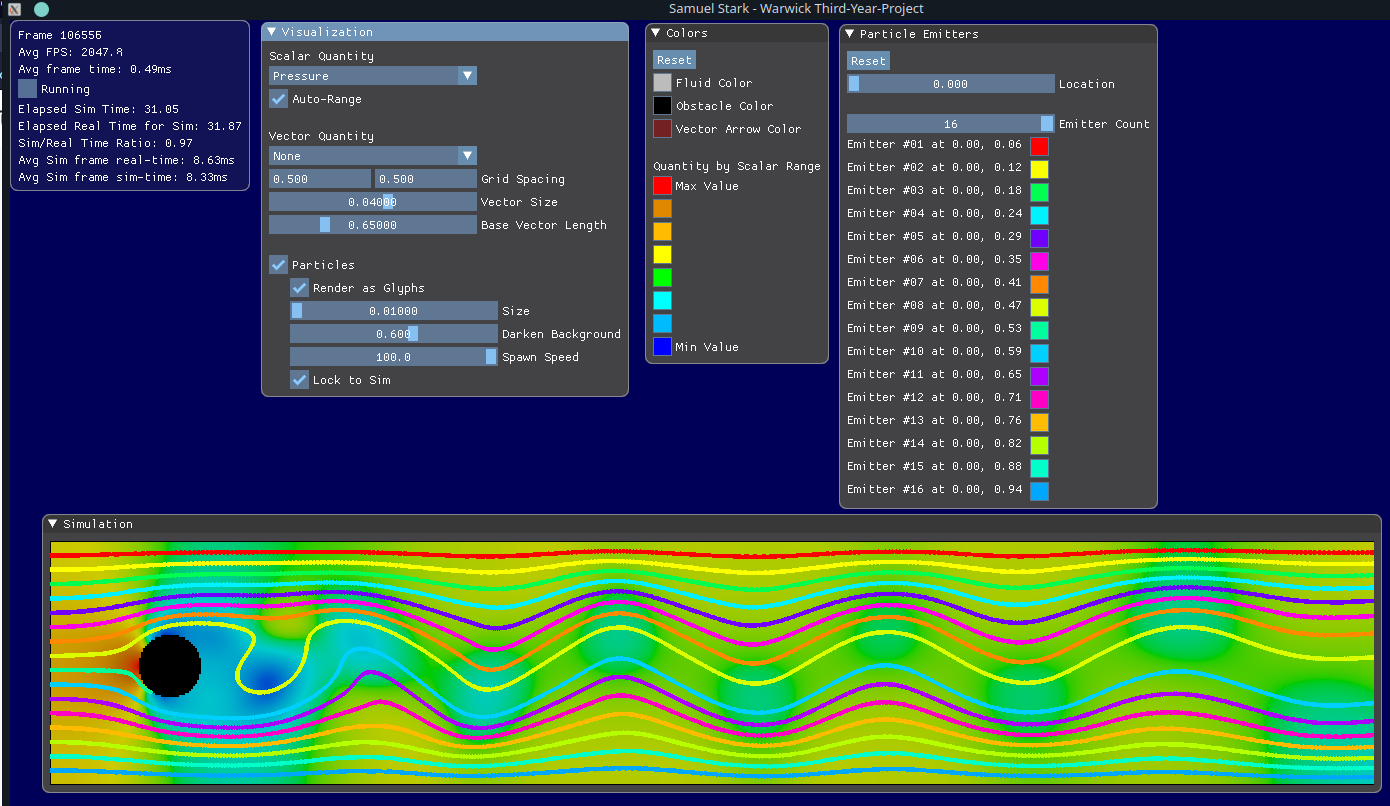
\includegraphics[width=0.8\textwidth]{Presentation/images/dan.png}
}
\end{frame}
\section{Evaluation}

\begin{frame}{GPU Utilization}
    % \todomark{Show profiler utilization}
    %     % TODO may need to use event synch to get profiler to look better for utilization
    % % https://on-demand.gputechconf.com/gtc/2014/presentations/S4158-cuda-streams-best-practices-common-pitfalls.pdf
    % % page 64
    
    \begin{wideitemize}
        \item GPU Utilization is close to 100\% where possible.
    
        \item At tick boundaries some bubbles appear as the CPU calculates the next $\delta{t}$.
    
        \item When visualizing, the Vulkan work hides this.
    \end{wideitemize}

    \vfill\null
    \begin{minipage}{0.49\textwidth}
        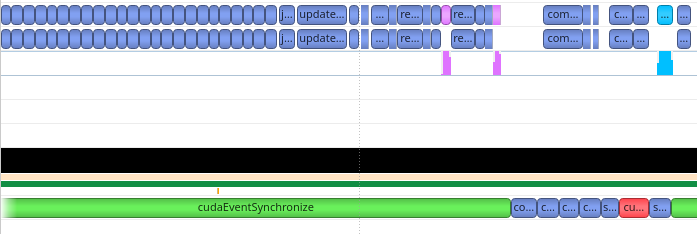
\includegraphics[width=\textwidth]{Presentation/images/sim_tick_edge.png}
        \begin{center}
            Tick Boundary
        \end{center}
    \end{minipage}\hfill%
    \begin{minipage}{0.49\textwidth}
        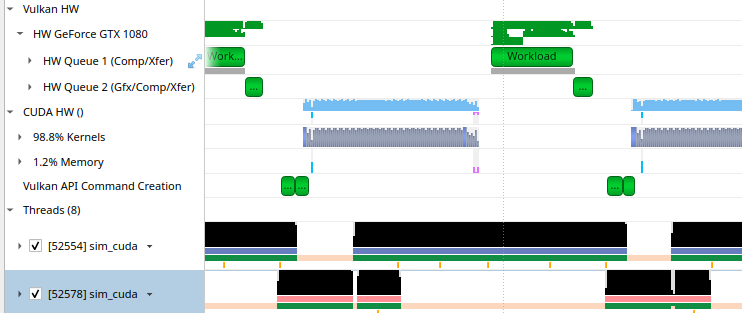
\includegraphics[width=\textwidth]{Presentation/images/final_pipeline_implementation.png}
        \begin{center}
            {Overall Visualization Pipeline}
        \end{center}
    \end{minipage}%\hfill%
    % \begin{minipage}{0.3\textwidth}
    
    % \end{minipage}
\end{frame}

\begin{frame}{Speed}
    % \todomark{Show graph of speed vs size for headless}
    % Speedup increases with longer running times for DETAILED ONLY
    % Speedup for ACA is constant w.r.t. accuracy
    % Speedup for large decreases w.r.t accuracy
    % Mean speedup at 2.3x vs. adapted ACA
    % ALL SPEEDUPS WITHIN [1.76, 2.77]
    
    \begin{wideitemize}
        \item Simulates the original CS257 input 2.47-2.86x faster than the original code.
        \item Visualization takes ~1.35ms per frame (740 FPS) at highest iteration count $N = 1000$
        % \footnote{When simulating at 120Hz. When simulating on every frame hits 170 FPS.}
        \item Individual visualization features are quick, and combined take less time than the simulation.\footnote{All points measured here in worst-case: with auto-range on where possible, and with maximum particles onscreen.}
    \end{wideitemize}
    
    \vfill\null
    
    \makebox[\textwidth][c]{
    {\renewcommand{\arraystretch}{1.5}%
    \begin{tabular}{|r|S[table-format=1.2,retain-explicit-plus]|S[table-format=1.2,retain-explicit-plus]|S[table-format=1.2,retain-explicit-plus]|S[table-format=1.2,retain-explicit-plus]|S[table-format=1.2,retain-explicit-plus]|}
    \hline
        & {Base Frame} & {with Sim} & {Scalar Quantity} & {Vector Field} & {Particles} \\ 
    \hline
        Mean Time (\si{\milli\second}) & 0.30 & 1.18 & 0.39 & 0.46 & 0.42 \\
        $\triangle$ from base (\si{\milli\second}) & {-} & +0.88 & +0.09 & +0.16 & +0.12 \\ 
    \hline
    \end{tabular}
    }
    }
    % \todomark{FPS above 120 for both normal and detailed profiles}
    % \todomark{Show approx time taken for each viz feature}
\end{frame}

\begin{frame}{Difference vs. Original}
    % \todomark{Created a tool to check accuracy against expected data}
    % \todomark{Using the same simulation profile (same iteration count etc.) got within 1E-11}
    \begin{wideitemize}
        \item The program contains a comparison tool for checking similarity.
    
        \item Simulating the original CS257 test has a mean square error of $10^{-14}$ for velocities, and $10^{-9}$ for pressure. 
    
        \item As iteration count and simulation time increases, the error becomes larger.
        \item Multiple potential causes in algorithm and implementation, but haven't researched further.
    \end{wideitemize}
    
    \vfill\null
    
    \makebox[\textwidth][c]{
    {\renewcommand{\arraystretch}{1.5}%
    % \begin{table}[t]
    %     \centering
        \begin{tabular}{|r|c|c|c|c|}
        \hline
            N & {100} & {200} & {300} & {1000} \\ 
        \hline
            Velocity MSE (u,v) & $10^{-14}$ & $10^{-14}$ & $10^{-14}$ & $10^{-14}$ \\
            Pressure MSE (p) & $10^{-9}$ & $10^{-8}$ & $10^{-7}$ & $10^{-6}$ \\
        \hline
        \end{tabular}
    % \end{table}
    }
    }
    \begin{center}
        Mean Square Error for original CS257 input data, simulated for \SI{10}{\second}
    \end{center}
\end{frame}

% Simulation is fast
% - inherent speedup moving from CPU to GPU
% - easy to get an accurate version working on CUDA
% - but wasn't a one/done process - needed to be aware of CUDA best practices and features to get speedups.
% - in ACA case and high-res case runs faster than real-time, faster than CPU version
% - but very dependent on simulation inputs.

% Simulation is accurate
% - results are close to ACA code
% - some differences because CUDA version doesn't use double-precision arithmetic, and uses FMAs more than ACA


% Visualization is fast
% - Particle sim and quantity-by-scalar elements add X time
% - Vector-quantity is oddly slow
% - 
\section{Project Management}
\begin{frame}{Project Management}
% \framesubtitle{Schedule}
    % \begin{minipage}{0.5\textwidth}
    %     % \setbeamertemplate{enumerate items}{\raisebox{-0.2em}{\scalebox{1.3}{\circled{\color{white}\insertenumlabel}}}}
    %     % \begin{enumerate}
    %     %     \itemsep1.3em
    %     %     \item Hadoop and MapReduce
    %     %     \item Apache Spark
    %     %     \item Spark SQL
    %     % \end{enumerate}
    %     This schedule was defined as part of the Specification document.
    % \end{minipage} \hfill
    % \begin{minipage}{0.49\textwidth}
    %     A particularly impactful element was the ``code freeze'' on Week 22.
        
    %     Sticking to this allowed me enough time to finish this presentation.
    %     % Otherwise it would not be done yet!
    % \end{minipage}
    \begin{wideitemize}
        \item Schedule defined as part of the Specification, planned for coding and writing reports.
        \item Code Freeze on Week 22 was very helpful
        \item Gave me enough time to finish the presentation!
    \end{wideitemize}
    
    \vfill\null
    \begin{tikzpicture}
        \node[inner sep=0pt] (gantt) at (0,0)
    {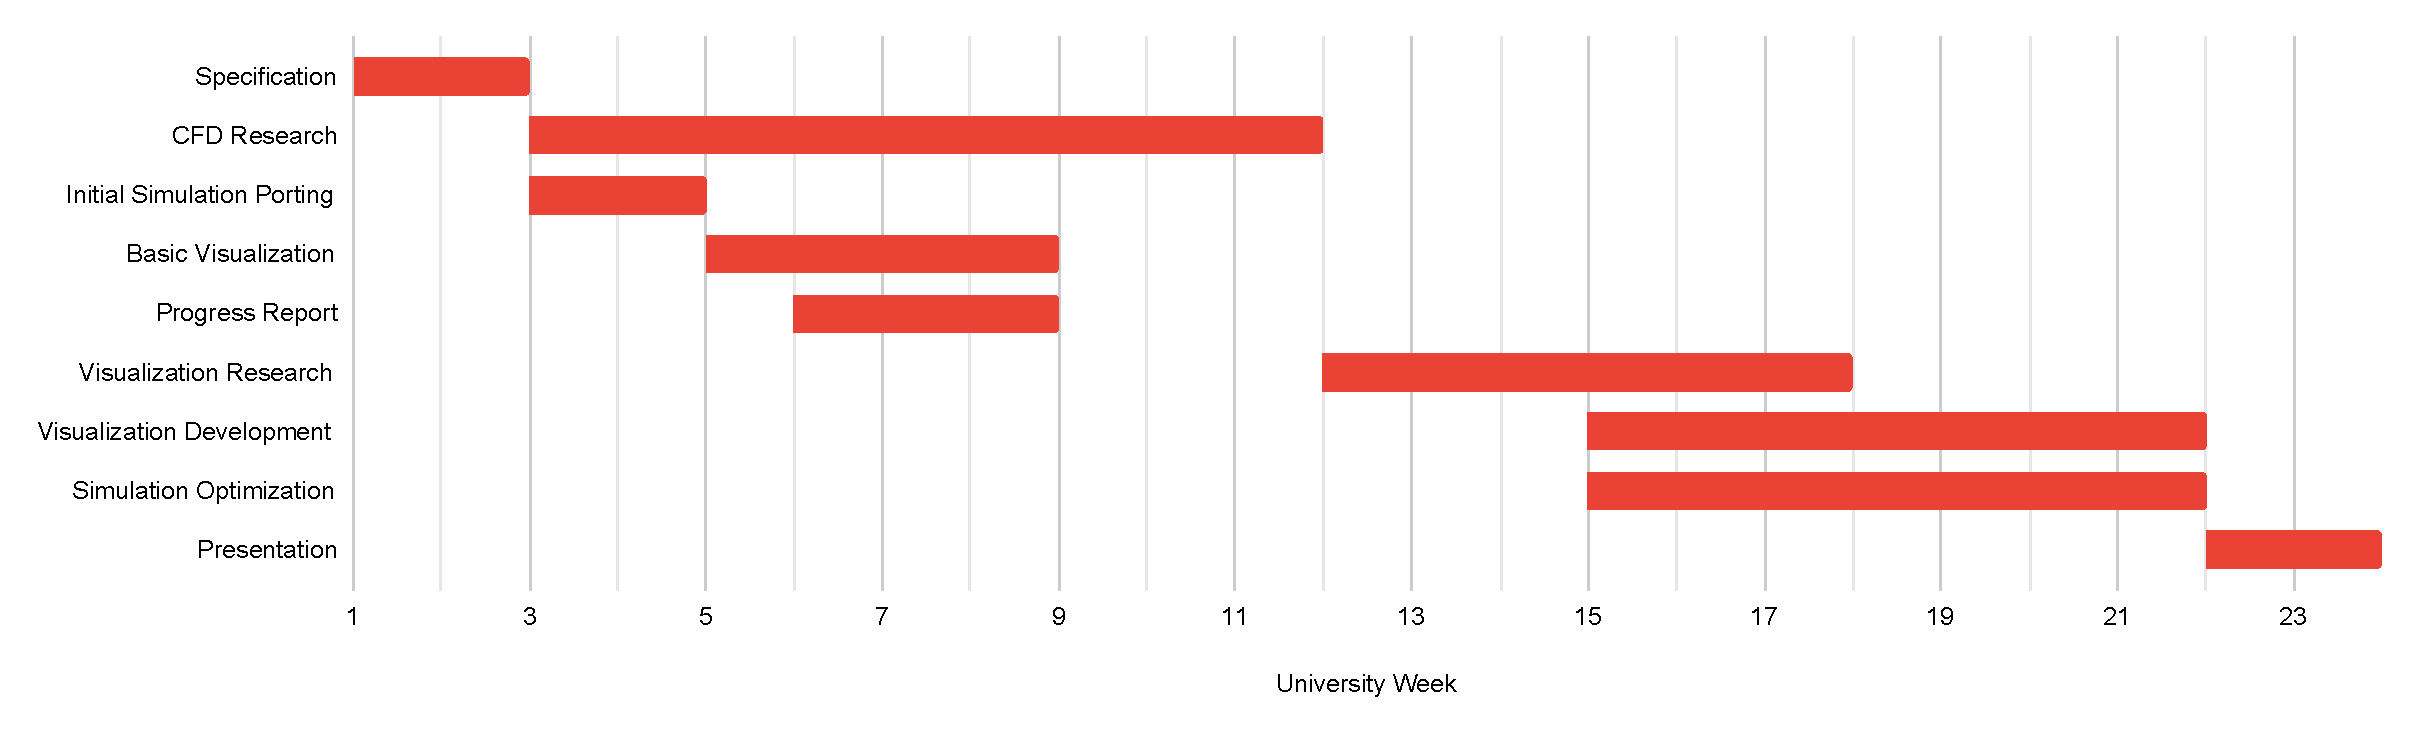
\includegraphics[width=1.0\linewidth]{Presentation/presentation_gantt.pdf}};
        \draw[line width=0.5mm] (5.4, -1.25) -- ++(0, 3) node[anchor=north east,align=right,fill=white] {Code Freeze};
        \node[text width=1.2cm,minimum height=2.35cm,fill opacity=0.5, fill=gray, font=\small,align=center, text opacity=1] at (-0.1,-0.02) {Christmas break and other work};
    \end{tikzpicture}
\end{frame}

% \begin{frame}{Project Management}
% \framesubtitle{Tools}
%     % C++17 + GCC 8
%     % CMake
%     % CUDA N
%     % vulkan.hpp
%     % Dear ImGui
%     % stb_image
% \end{frame}
\section{Conclusion \& Future Work}
\begin{frame}{Conclusion}
    % \todomark{Conclusion}
    % 8.5Kloc over 164 files, not including external libraries, comments, or blanks.
% 52 lines per file on avg?
% For C/C++, 132/file on average
% For headers, 30/file
% For CUDA, 51/file (probs counts CUDA headers)
% GLSL, 40/file.

% \todomark{All goals acheived!}
% \begin{center}
%     All goals were achieved!
% \end{center}
% \vfill\null
\begin{wideitemize}
    \item Overall, the project was a success.
    \item CUDA is a very intuitive API, especially for those without prior compute experience.
    \item Vulkan requires more heavy lifting, but it seems to have been worth it.
    \item Looking to the games industry for advice in i.e. particle rendering is helpful.
    
    \item For the scientific community to start using Vulkan, simple abstraction layers will be needed.
    \begin{wideitemize}
        \item VTK, a popular visualization library, has a Vulkan branch that seems to be dead.
        \item Datoviz is a new library with Python bindings that renders with Vulkan.
    \end{wideitemize}
    
    \item CUDA-Vulkan interoperability is nice! Resources should be allocated from Vulkan to maintain full control.
\end{wideitemize}
\end{frame}

\begin{frame}{Future Work}
    Simulation
    \begin{wideitemize}
        \item Investigate simulation accuracy and algorithm.
        \item Re-introduce the Poisson accuracy check.
        \item Optimize parallel reductions.
    \end{wideitemize}
    \vfill\null
    Visualization
    \begin{wideitemize}
        \item Investigate colorblindness options.
        \item Better memory allocation, potentially using a helper library.
        \item Run different layer computations in parallel with separate command buffers?
    \end{wideitemize}
\end{frame}
\usebeamertemplate{endpage}

\begin{frame}[allowframebreaks]{References}
\def\newblock{}
\begingroup
\raggedright
% \printbibheading[heading=bibnumbered]
% #1
\printbibliography[]
\endgroup
\end{frame}

\section*{Extras}
\appendsubframes

\end{document} 